\documentclass[12pt,english,dvipsnames,aspectratio=169,handout]{beamer}\usepackage[]{graphicx}\usepackage[]{xcolor}
% maxwidth is the original width if it is less than linewidth
% otherwise use linewidth (to make sure the graphics do not exceed the margin)
\makeatletter
\def\maxwidth{ %
  \ifdim\Gin@nat@width>\linewidth
    \linewidth
  \else
    \Gin@nat@width
  \fi
}
\makeatother

\definecolor{fgcolor}{rgb}{0.345, 0.345, 0.345}
\newcommand{\hlnum}[1]{\textcolor[rgb]{0.686,0.059,0.569}{#1}}%
\newcommand{\hlstr}[1]{\textcolor[rgb]{0.192,0.494,0.8}{#1}}%
\newcommand{\hlcom}[1]{\textcolor[rgb]{0.678,0.584,0.686}{\textit{#1}}}%
\newcommand{\hlopt}[1]{\textcolor[rgb]{0,0,0}{#1}}%
\newcommand{\hlstd}[1]{\textcolor[rgb]{0.345,0.345,0.345}{#1}}%
\newcommand{\hlkwa}[1]{\textcolor[rgb]{0.161,0.373,0.58}{\textbf{#1}}}%
\newcommand{\hlkwb}[1]{\textcolor[rgb]{0.69,0.353,0.396}{#1}}%
\newcommand{\hlkwc}[1]{\textcolor[rgb]{0.333,0.667,0.333}{#1}}%
\newcommand{\hlkwd}[1]{\textcolor[rgb]{0.737,0.353,0.396}{\textbf{#1}}}%
\let\hlipl\hlkwb

\usepackage{framed}
\makeatletter
\newenvironment{kframe}{%
 \def\at@end@of@kframe{}%
 \ifinner\ifhmode%
  \def\at@end@of@kframe{\end{minipage}}%
  \begin{minipage}{\columnwidth}%
 \fi\fi%
 \def\FrameCommand##1{\hskip\@totalleftmargin \hskip-\fboxsep
 \colorbox{shadecolor}{##1}\hskip-\fboxsep
     % There is no \\@totalrightmargin, so:
     \hskip-\linewidth \hskip-\@totalleftmargin \hskip\columnwidth}%
 \MakeFramed {\advance\hsize-\width
   \@totalleftmargin\z@ \linewidth\hsize
   \@setminipage}}%
 {\par\unskip\endMakeFramed%
 \at@end@of@kframe}
\makeatother

\definecolor{shadecolor}{rgb}{.97, .97, .97}
\definecolor{messagecolor}{rgb}{0, 0, 0}
\definecolor{warningcolor}{rgb}{1, 0, 1}
\definecolor{errorcolor}{rgb}{1, 0, 0}
\newenvironment{knitrout}{}{} % an empty environment to be redefined in TeX

\usepackage{alltt}
\usepackage{fontspec}
\setsansfont[Mapping=tex-text]{Fira Sans}
\setcounter{secnumdepth}{4}
\setcounter{tocdepth}{4}
\usepackage[normalem]{ulem}
\usepackage[T1]{fontenc}
\usepackage{dcolumn}
\usepackage{booktabs}
\usepackage{bm}
\usepackage{setspace}
\makeatletter
\usetheme{metropolis}
\setbeamertemplate{frame footer}{Bosancianu | Schaub | Hertie School}
\setbeamerfont{page number in head/foot}{size=\tiny}
\setbeamercolor{footline}{fg=gray}
\usepackage{xcolor}
\setbeamercovered{dynamic}
\usepackage{tikz}
\usetikzlibrary{arrows, positioning,fit,shapes.misc}
\usepackage[labelformat=empty]{caption}
% For table captions in Beamer
\usepackage[sectionbib]{apacite}
\renewcommand{\bibliographytypesize}{\footnotesize}
\makeatletter
\let\st@rtbibsection\@bibnewpage
\let\st@rtbibchapter\@bibnewpage
\makeatother
\usepackage{amsmath, mathtools}
\usepackage{xunicode}
\usepackage{hyperref}
\graphicspath{{./figures/}} 
% Defines a checkmark
\def\checkmark{\tikz\fill[scale=0.4,color=orange](0,.35) -- (.25,0) -- (1,.7) -- (.25,.15) -- cycle;}
\newcommand{\indep}{\perp \!\!\!\! \perp}
\setbeamertemplate{itemize items}{\checkmark}
\usepackage{multirow}
\hypersetup{pdfauthor={Bosancianu and Schaub},
	pdftitle={Statistical Modeling and Causal Inference with R},
	pdfsubject={Week 7: Regression Discontinuity Designs},
	pdfkeywords={Berlin, Hertie, 2020, week 7, RDD}}
% FOR UNIFORM DENSITY
\usepackage{pgfplots}
\makeatletter
\long\def\ifnodedefined#1#2#3{%
    \@ifundefined{pgf@sh@ns@#1}{#3}{#2}%
}
\pgfplotsset{
    discontinuous/.style={
    scatter,
    scatter/@pre marker code/.code={
        \ifnodedefined{marker}{
            \pgfpointdiff{\pgfpointanchor{marker}{center}}%
             {\pgfpoint{0}{0}}%
             \ifdim\pgf@y>0pt
                \tikzset{options/.style={mark=*}}
                \draw [densely dashed] (marker-|0,0) -- (0,0);
                \draw plot [mark=*,mark options={fill=white}] coordinates {(marker-|0,0)};
             \else
                \ifdim\pgf@y<0pt
                    \tikzset{options/.style={mark=*,fill=white}}
                    \draw [densely dashed] (marker-|0,0) -- (0,0);
                    \draw plot [mark=*] coordinates {(marker-|0,0)};
                \else
                    \tikzset{options/.style={mark=none}}
                \fi
             \fi
        }{
            \tikzset{options/.style={mark=none}}        
        }
        \coordinate (marker) at (0,0);
        \begin{scope}[options]
    },
    scatter/@post marker code/.code={\end{scope}}
    }
}
\makeatother
\title{\textsc{Statistical Modeling and Causal Inference with R}}
\subtitle{Week 7: Regression Discontinuity Designs}
\date{October 26, 2020}
\author{Manuel Bosancianu \hfill Max Schaub}
\institute{Hertie School of Governance}
\IfFileExists{upquote.sty}{\usepackage{upquote}}{}
\begin{document}
\maketitle




\section{Introduction}

\begin{frame}
\frametitle{RDD features}

\begin{itemize}
\item a score / running variable / forcing variable / index
\item a cutoff / threshold
\item a treatment
\end{itemize}
\pause
\bigskip

$P_{assignment}$ changes discontinuously at the threshold.

\end{frame}


\begin{frame}
\frametitle{Sharp RDD}
The \citeA{fujiwara_voting_2015} study is an example of \textit{sharp} RDD:

\begin{itemize}
  \item all 307 municipalities above 40,500 registered voters used EV
  \item 4,967 out of 4,974 municipalities below 40,500 registered voters used paper ballots
\end{itemize}
\pause
\bigskip

\begin{equation}
  \tau = \lim_{\upsilon_m \downarrow 40,500}E[Y_m | \upsilon_m] - \lim_{\upsilon_m \uparrow 40,500}E[Y_m | \upsilon_m]
  \label{eq:01}
\end{equation}


\end{frame}


 
\begin{frame}
\frametitle{Estimating RD effects}

\begin{columns}
	\begin{column}{0.35\textwidth}
	Uses linear regressions, without any weights (``rectangular'' kernel).\bigskip
	
	Here, $c=0$ and $h=1$.
	\end{column}
	\begin{column}{0.65\textwidth}
		\begin{tikzpicture}[
    declare function={unipdf(\x,\xl,\xu)= (\x>=\xl)*(\x<\xu)*1/(\xu-\xl);},
    scale = 0.9]

\begin{axis}[
    samples=11,
    jump mark left,
    ymin=0,ymax=1,
    xmin=-5, xmax=5,
    every axis plot/.style={very thick},
    discontinuous
]
\addplot [orange] {unipdf(x,-1,1)};
\end{axis}
\end{tikzpicture}
	\end{column}
\end{columns}

\end{frame}


\begin{frame}
\frametitle{Estimating RD effects}
Assume that:

$V_m$ are the registered voters in municipality $m$, and that

\begin{equation}
D = \begin{cases}
0, & if\; V_m < 40,500 \\
1, & if\; V_m \geq 40,500 
\end{cases}
\label{eq:02}
\end{equation}

\begin{equation}
Y_m = \beta_0 + \tau D_m + \beta_1V_m + \beta_2V_mD_m + \epsilon_m  
  \label{eq:03}
\end{equation}
\pause

What kind of regression \textcolor{orange}{characteristics} is this assuming? What  \textcolor{orange}{assumptions} are implicit? 
\end{frame}


\begin{frame}
\frametitle{Linear model \& different slope}

\begin{figure}
\centering
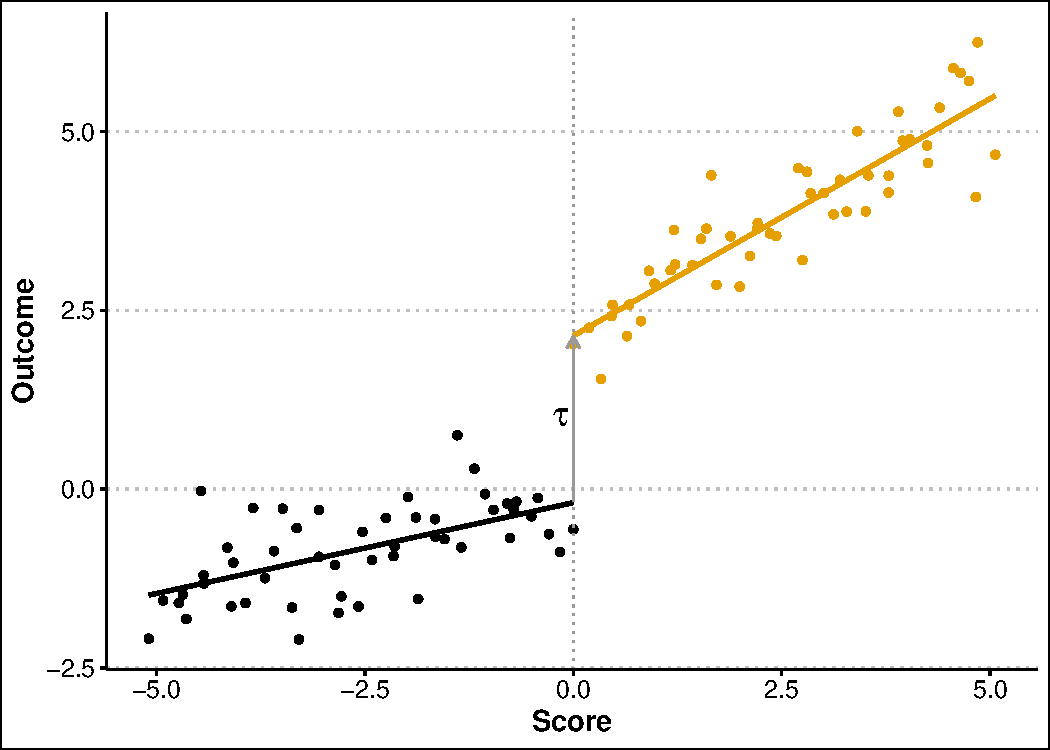
\includegraphics[scale=0.35]{../04-figures/07/10.pdf}
\end{figure}
\pause

\begin{itemize}
\footnotesize
\item linearity: regressions are linear in $V_m$
\item varying treatment effect ($\tau$) along $V$
\end{itemize}

\end{frame}


\section{Results}

\begin{frame}
\frametitle{Is there a jump at cutoff?}

\begin{figure}
\centering
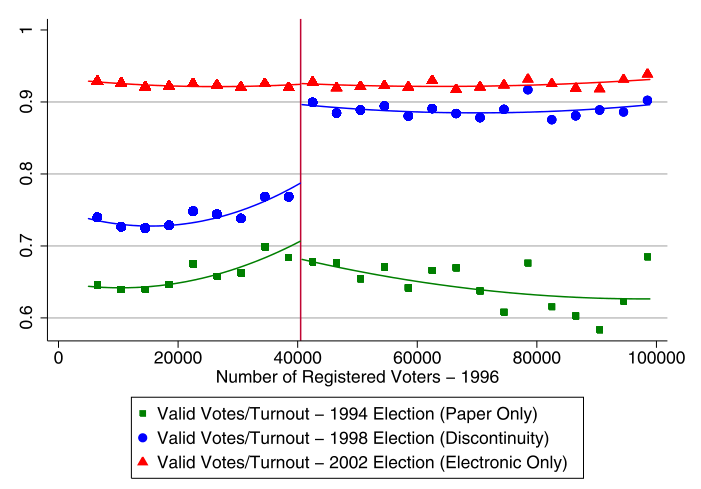
\includegraphics[scale=0.4]{../04-figures/07/19.PNG}
\caption{Figure 2 (p.~435)}
\end{figure}

Why are the other two election years provided here?
\end{frame}


\begin{frame}
\frametitle{Effect of introducing EV}

\begin{figure}
\centering
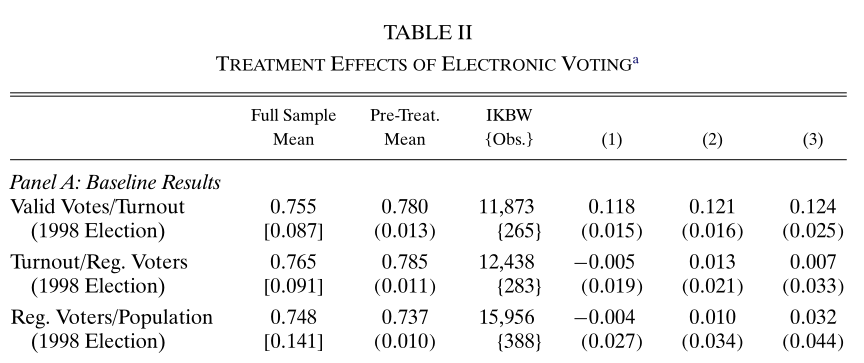
\includegraphics[scale=0.4]{../04-figures/07/20-1.PNG}
\caption{Table 2 (p.~436)}
\end{figure}

\end{frame}


\begin{frame}
\frametitle{Placebo tests}

\begin{figure}
\centering
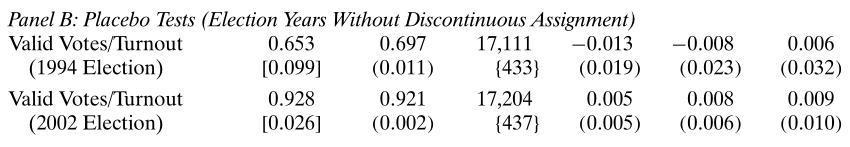
\includegraphics[scale=0.4]{../04-figures/07/20-2.PNG}
\caption{Table 2 (p.~436)}
\end{figure}

\end{frame}


\begin{frame}
\frametitle{Parties favored}

\begin{figure}
\centering
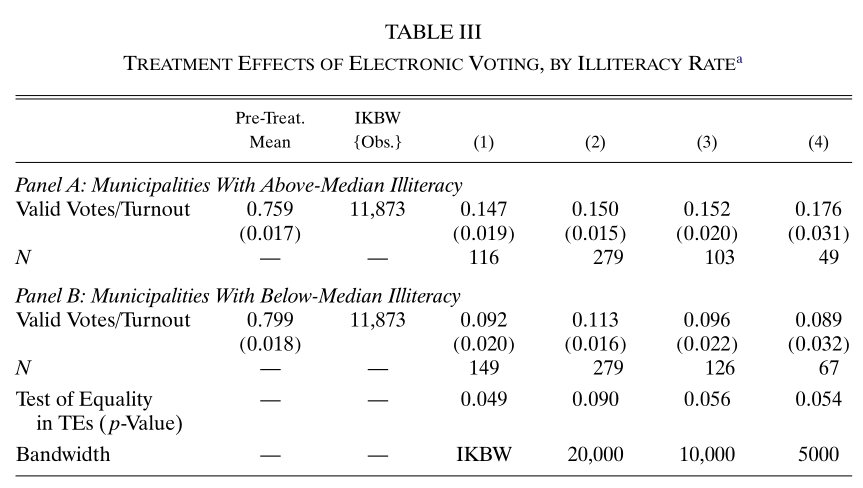
\includegraphics[scale=0.4]{../04-figures/07/22.PNG}
\caption{Table 3 (p.~439)}
\end{figure}

\end{frame}

\section{Validity checks}
 
\begin{frame}
\frametitle{Falsification and validity}

What were the 5 types of \textcolor{orange}{falsification} and \textcolor{orange}{validity} tests?\pause
\bigskip

\begin{enumerate}
\item null effect on pre-treatment covariates and placebo outcomes
\item score density continuity around cutoff
\item treatment effect at artificial cutoff values
\item excluding observations near cutoff
\item sensitivity to bandwidth choices
\end{enumerate}
\end{frame}


\begin{frame}
\frametitle{Bandwidth sensitivity}

\begin{figure}
\centering
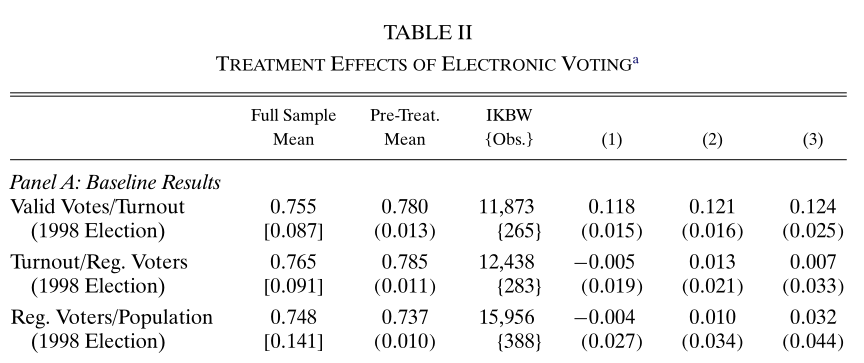
\includegraphics[scale=0.4]{../04-figures/07/20-1.PNG}
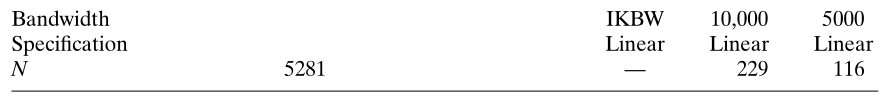
\includegraphics[scale=0.48]{../04-figures/07/20-3.PNG}
\caption{Table 2 (p.~436)}
\end{figure}

\end{frame}


\begin{frame}
\frametitle{Null effect on pre-treatment covariates}

\begin{figure}
\centering
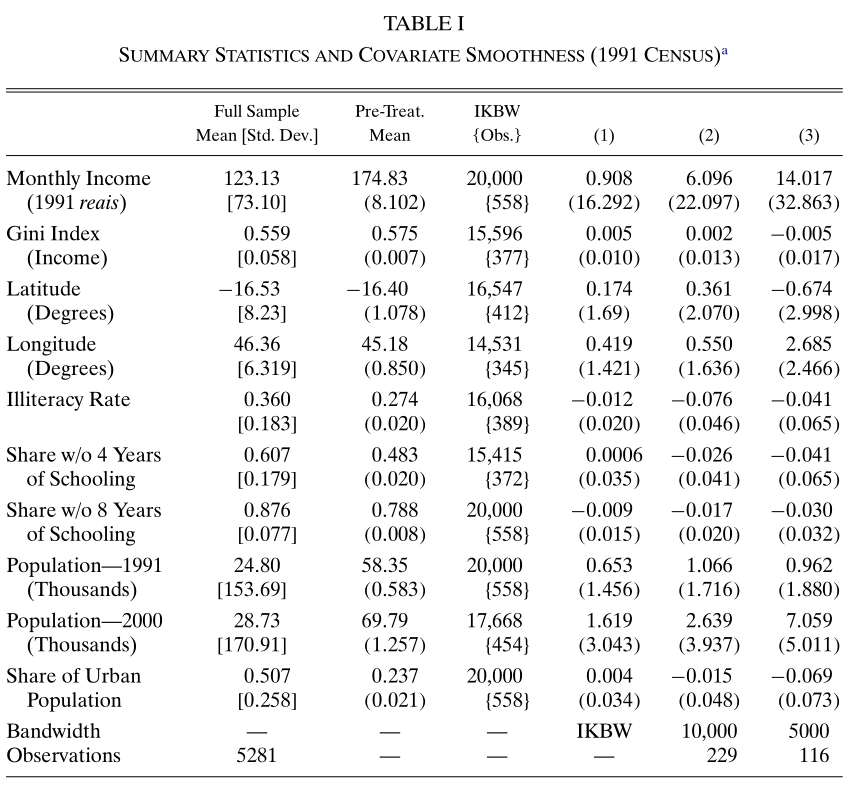
\includegraphics[scale=0.3]{../04-figures/07/21.PNG}
\caption{Table 1 (p.~434)}
\end{figure}

\end{frame}

\begin{frame}
\frametitle{Score density around cutoff}

\begin{columns}
	\begin{column}{0.35\textwidth}
	Danger here is that we may be dealing with sorting.\bigskip
	
	Discussed in text as implausible---\textcolor{orange}{why?}
	\end{column}\pause
	\begin{column}{0.65\textwidth}
		\begin{figure}
    \centering
    \visible<2>{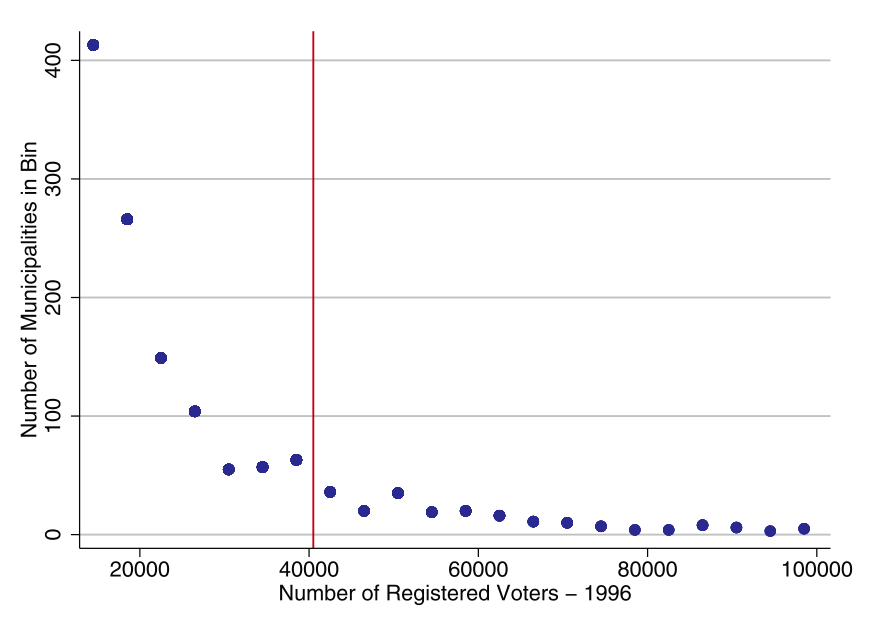
\includegraphics[scale=0.4]{../04-figures/07/23.PNG}}
    \visible<2>{\caption{Figure A2}}
    \end{figure}
	\end{column}
\end{columns}


\end{frame}


\begin{frame}[fragile]
\frametitle{Score density: testing}







\begin{table}
\centering
\footnotesize
\caption{Number of cases in bins}
\begin{tabular}{l c}
\toprule
  Registered voters & N \\
\midrule
28,500-32,500 & 55 \\
32,500-36,500 & 57 \\
36,500-40,500 & 63 \\
40,500-44,500 & 36 \\
44,500-48,500 & 20 \\
48,500-52,500 & 35 \\
\bottomrule
\end{tabular}
\label{tab:01}
\end{table}
\pause

\begin{knitrout}
\definecolor{shadecolor}{rgb}{0.969, 0.969, 0.969}\color{fgcolor}\begin{kframe}
\begin{alltt}
\hlkwd{binom.test}\hlstd{(}\hlnum{36}\hlstd{,} \hlnum{99}\hlstd{,} \hlkwc{p} \hlstd{=} \hlnum{0.5}\hlstd{)}
\end{alltt}
\end{kframe}
\end{knitrout}

\end{frame}


\begin{frame}[fragile]
\frametitle{Score density: testing}

{\tiny
\begin{knitrout}
\definecolor{shadecolor}{rgb}{0.969, 0.969, 0.969}\color{fgcolor}\begin{kframe}
\begin{verbatim}

	Exact binomial test

data:  36 and 99
number of successes = 36, number of trials = 99, p-value = 0.008634
alternative hypothesis: true probability of success is not equal to 0.5
95 percent confidence interval:
 0.2692701 0.4663956
sample estimates:
probability of success 
             0.3636364 
\end{verbatim}
\end{kframe}
\end{knitrout}
}\pause

Argument about timing of EV announcement cutoff is more convincing.

\end{frame}


\begin{frame}[fragile]
\frametitle{Artificial cutoffs}
What was the logic here?\bigskip
\pause



\begin{figure}
\centering
\visible<2>{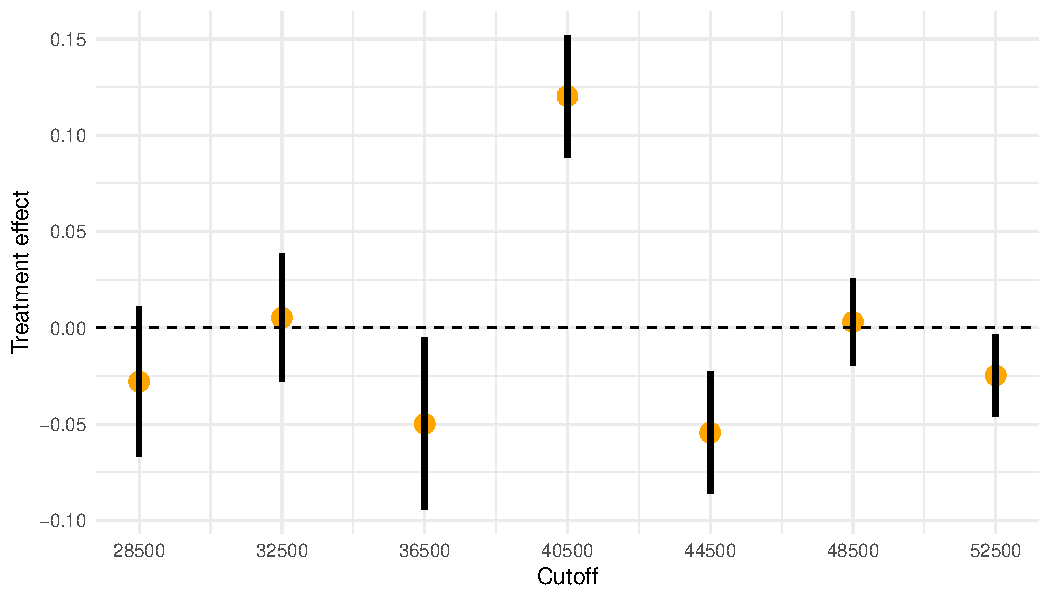
\includegraphics[scale=0.5]{../04-figures/07/24.pdf}}
\end{figure}

\end{frame}


\begin{frame}
\frametitle{``Doughnut hole'' test}
What was the logic here?\bigskip
\pause

I re-ran the model with gradually eliminating municipalities in bins of 500 registered voters on either side of cutoff.



\end{frame}

\begin{frame}
\frametitle{``Doughnut hole'' test}

\begin{figure}
\centering
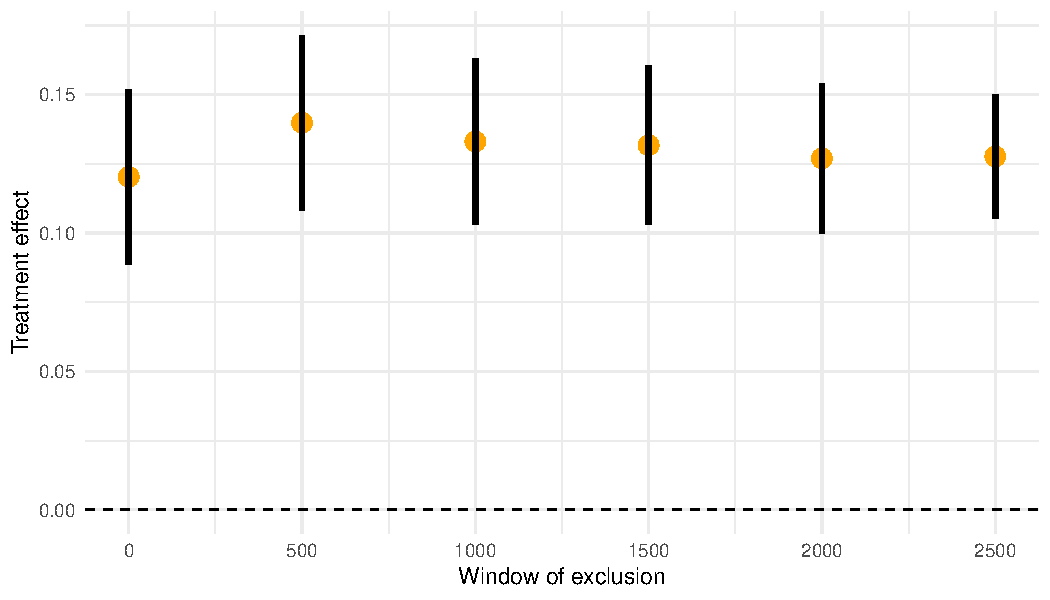
\includegraphics[scale=0.6]{../04-figures/07/25.pdf}
\end{figure}

\end{frame}


% END
\begin{frame}
\begin{center}
    \Huge Thank \textcolor{orange}{you} for the kind attention!
\end{center}
\end{frame}

% REFERENCES %

\begin{frame}[allowframebreaks]
\bibliographystyle{apacite}
\scriptsize\bibliography{../Bibliography}
\end{frame}

\end{document}
